\documentclass[12pt, twoside]{article}
%\documentclass[12pt, twoside]{article}
\usepackage[letterpaper, margin=1in, headsep=0.2in]{geometry}
\setlength{\headheight}{0.6in}
%\usepackage[english]{babel}
\usepackage[utf8]{inputenc}
\usepackage{microtype}
\usepackage{amsmath}
\usepackage{amssymb}
%\usepackage{amsfonts}
\usepackage[nomessages]{fp} %\FPeval{\var-name}{2*sin(pi/6)}
\usepackage{siunitx} %units in math. eg 20\milli\meter
\usepackage{yhmath} % for arcs, overparenth command
\usepackage{tikz} %graphics
\usetikzlibrary{quotes, angles, arrows, arrows.meta}
\usepackage{pgfplots}
\usepgfplotslibrary{fillbetween}
\pgfplotsset{compat=1.16}
\usepackage{graphicx} %consider setting \graphicspath{{images/}}
\usepackage{parskip} %no paragraph indent
\usepackage{enumitem}
\usepackage{multicol}
\usepackage{venndiagram}

\usepackage{fancyhdr}
\pagestyle{fancy}
\fancyhf{}
\renewcommand{\headrulewidth}{0pt} % disable the underline of the header
\raggedbottom
\hfuzz=2mm %suppresses overfull box warnings

\usepackage{hyperref}

\fancyhead[LO]{La Scuola d'Italia / Dr.\ Huson / IB Math 12 \\* 10 November 2026}
\fancyhead[RO]{\fbox{\begin{minipage}{6cm}\footnotesize Nickname:\\[0.5cm]\end{minipage}}}
\fancyfoot[C]{\thepage}

\begin{document}
\subsubsection*{1.12 Classwork: Simpson's Paradox --- correlating levels and changes}

\emph{Use your GDC. Give answers correct to three significant figures.
Data: monthly averages, January 2003 to December 2011 (sources: FRED,
OECD).}

\begin{center}
\fbox{\begin{minipage}{0.94\textwidth}
\textbf{An Italian investor in US bonds.} In January 2003 an investor in
Milan changes EUR $100\,000$ into US dollars and buys US 10-year government
bonds (Treasuries). The investment carries two risks.
\begin{itemize}[itemsep=0pt, topsep=2pt]
  \item \textbf{Interest-rate risk.} When the US 10-year \emph{yield}
  rises, the price of bonds already issued falls.
  \item \textbf{Currency risk.} The investor will change the dollars back
  into euros. The exchange rate EUR/USD is the number of US dollars that
  one euro buys. A \emph{higher} EUR/USD means a \emph{weaker} dollar.
\end{itemize}
\end{minipage}}
\end{center}

\begin{enumerate}[itemsep=0.15cm]

%--- Problem 1: Reading the two time series; currency conversion in and out of dollars; effect of a weaker and a stronger dollar on the investor ---
%--- Source: Original (AA SL 1.4, 4.1 context); data FRED IRLTLT01USM156N and EXUSEU, see claude-ib-project/output/correlation_claude ---
\item[1.] The graph shows the US 10-year yield (solid line, left scale)
and EUR/USD (dashed line, right scale) for each month.

\begin{center}
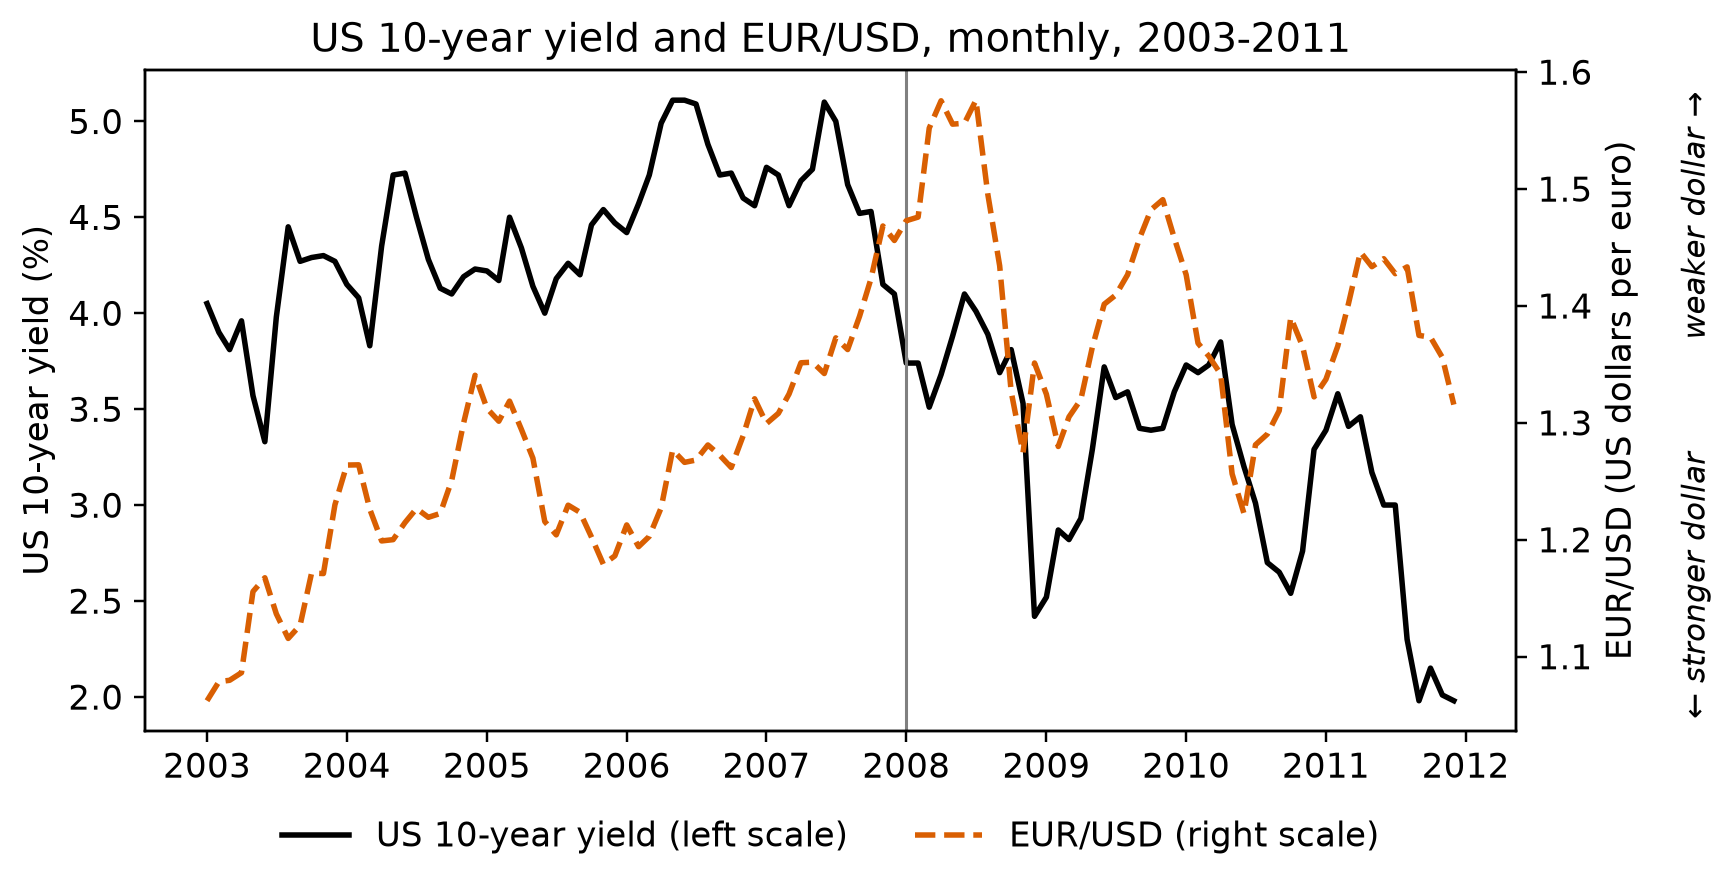
\includegraphics[width=0.82\textwidth]{../graphics/1-12CW_D_eurusd_us10y_1_timeseries.png}
\end{center}

\begin{center}
\setlength{\tabcolsep}{6pt}\renewcommand{\arraystretch}{1.15}
\begin{tabular}{|l|c|c|c|c|}
\hline
Month & Jan 2003 & Jul 2008 & Nov 2008 & Dec 2008 \\
\hline
US 10-year yield (\%) & 4.05 & 4.01 & 3.53 & 2.42 \\
\hline
EUR/USD & 1.0622 & 1.5759 & 1.2744 & 1.3511 \\
\hline
\end{tabular}
\end{center}

\begin{enumerate}[itemsep=0.1cm]
  \item Find the number of US dollars the investor receives for
  EUR $100\,000$ in January 2003.
  \vfill
  \item Ignoring interest and any change in the bond price, find the value
  of these dollars in euros in July 2008. Find the percentage change from
  the investor's EUR $100\,000$.
  \vfill
  \item Did the dollar become stronger or weaker between July and November
  2008? Find the value in euros of the same dollars in November 2008.
  \vfill
  \item Describe the change in the US 10-year yield between July and
  December 2008. Explain whether this change was good or bad for the
  investor.
  \vfill
\end{enumerate}

\newpage

%--- Problem 2: Correlation of levels: r for each period and the whole period; Simpson's paradox explained by the shift in the period means ---
%--- Source: Original (AA SL 4.4); data set D of claude-ib-project/output/correlation_claude ---
\item[2.]

Each point in the scatter diagram is one month: the US 10-year yield, $x$,
and EUR/USD, $y$. Circles are 2003--2007 and triangles are 2008--2011.

\begin{center}
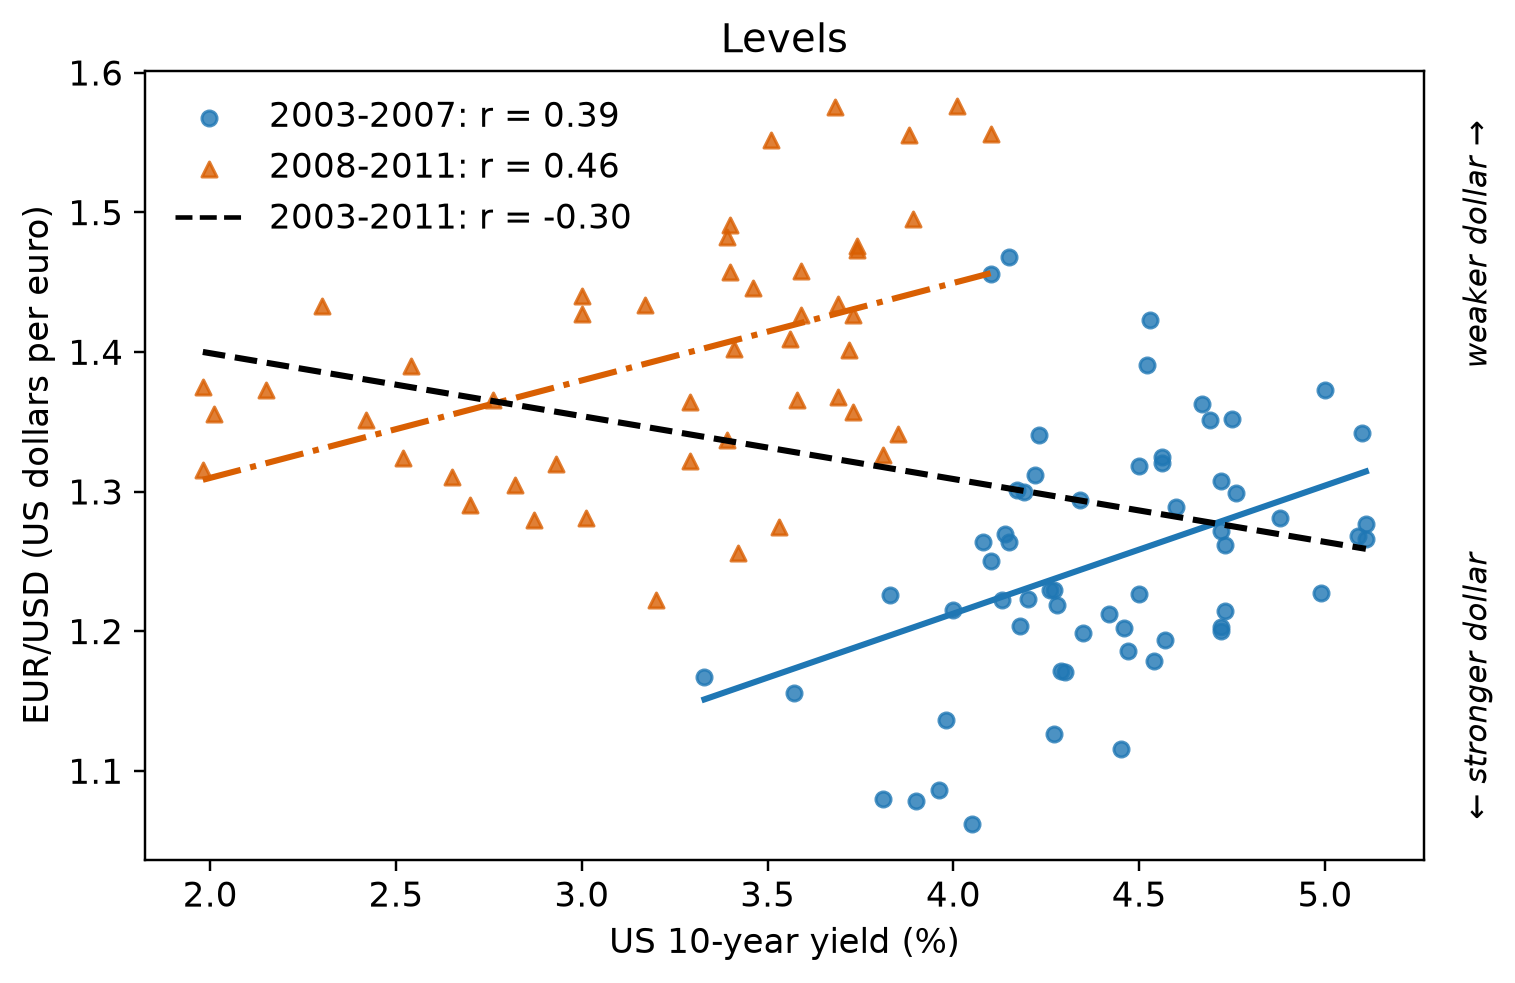
\includegraphics[width=0.74\textwidth]{../graphics/1-12CW_D_eurusd_us10y_2_levels_scatter.png}
\end{center}

\begin{center}
\setlength{\tabcolsep}{6pt}\renewcommand{\arraystretch}{1.15}
\begin{tabular}{|l|c|c|}
\hline
Period & mean yield, $\bar{x}$ (\%) & mean EUR/USD, $\bar{y}$ \\
\hline
2003--2007 (60 months) & 4.40 & 1.249 \\
\hline
2008--2011 (48 months) & 3.23 & 1.396 \\
\hline
\end{tabular}
\end{center}

\begin{enumerate}[itemsep=0.1cm]
  \item Write down the value of Pearson's $r$ for 2003--2007, for
  2008--2011, and for the whole period 2003--2011. Describe each
  correlation.
  \vfill
  \item Use the table of means to explain how the correlation can be
  positive in each period but negative for the two periods together.
  \vfill
  \item Simpson's paradox is a relationship that holds within each group
  but reverses when the groups are combined. A student concludes from the
  whole-period value of $r$: ``When US yields rise, the dollar gets
  stronger.'' Explain why this conclusion is not justified.
  \vfill
\end{enumerate}

\newpage

%--- Problem 3: Monthly changes: change in percentage points and percentage change; r of changes in each period; interpretation as a partial hedge for the investor ---
%--- Source: Original (AA SL 1.4, 4.4); data set D of claude-ib-project/output/correlation_claude ---
\item[3.]

Finance compares \emph{changes}, month to month. For the yield the change
is in percentage points; for the exchange rate it is the percentage change:
\[
  \text{change in yield} = x_{\text{this month}} - x_{\text{last month}},
  \qquad
  \text{change in EUR/USD} = \frac{y_{\text{this month}} - y_{\text{last month}}}{y_{\text{last month}}} \times 100.
\]

\begin{center}
\setlength{\tabcolsep}{5pt}\renewcommand{\arraystretch}{1.15}
\begin{tabular}{|l|c|c|c|c|c|c|}
\hline
Month (2008) & Jul & Aug & Sep & Oct & Nov & Dec \\
\hline
US 10-year yield (\%) & 4.01 & 3.89 & 3.69 & 3.81 & 3.53 & 2.42 \\
\hline
change (percentage points) & & $-0.12$ & & & & \\
\hline
EUR/USD & 1.5759 & 1.4955 & 1.4342 & 1.3266 & 1.2744 & 1.3511 \\
\hline
change (\%) & & $-5.10$ & & & & \\
\hline
\end{tabular}
\end{center}

\begin{enumerate}[itemsep=0.1cm]
  \item Complete the table.
  \vfill
\end{enumerate}

The scatter diagram shows the monthly changes for all 108 months.

\begin{center}
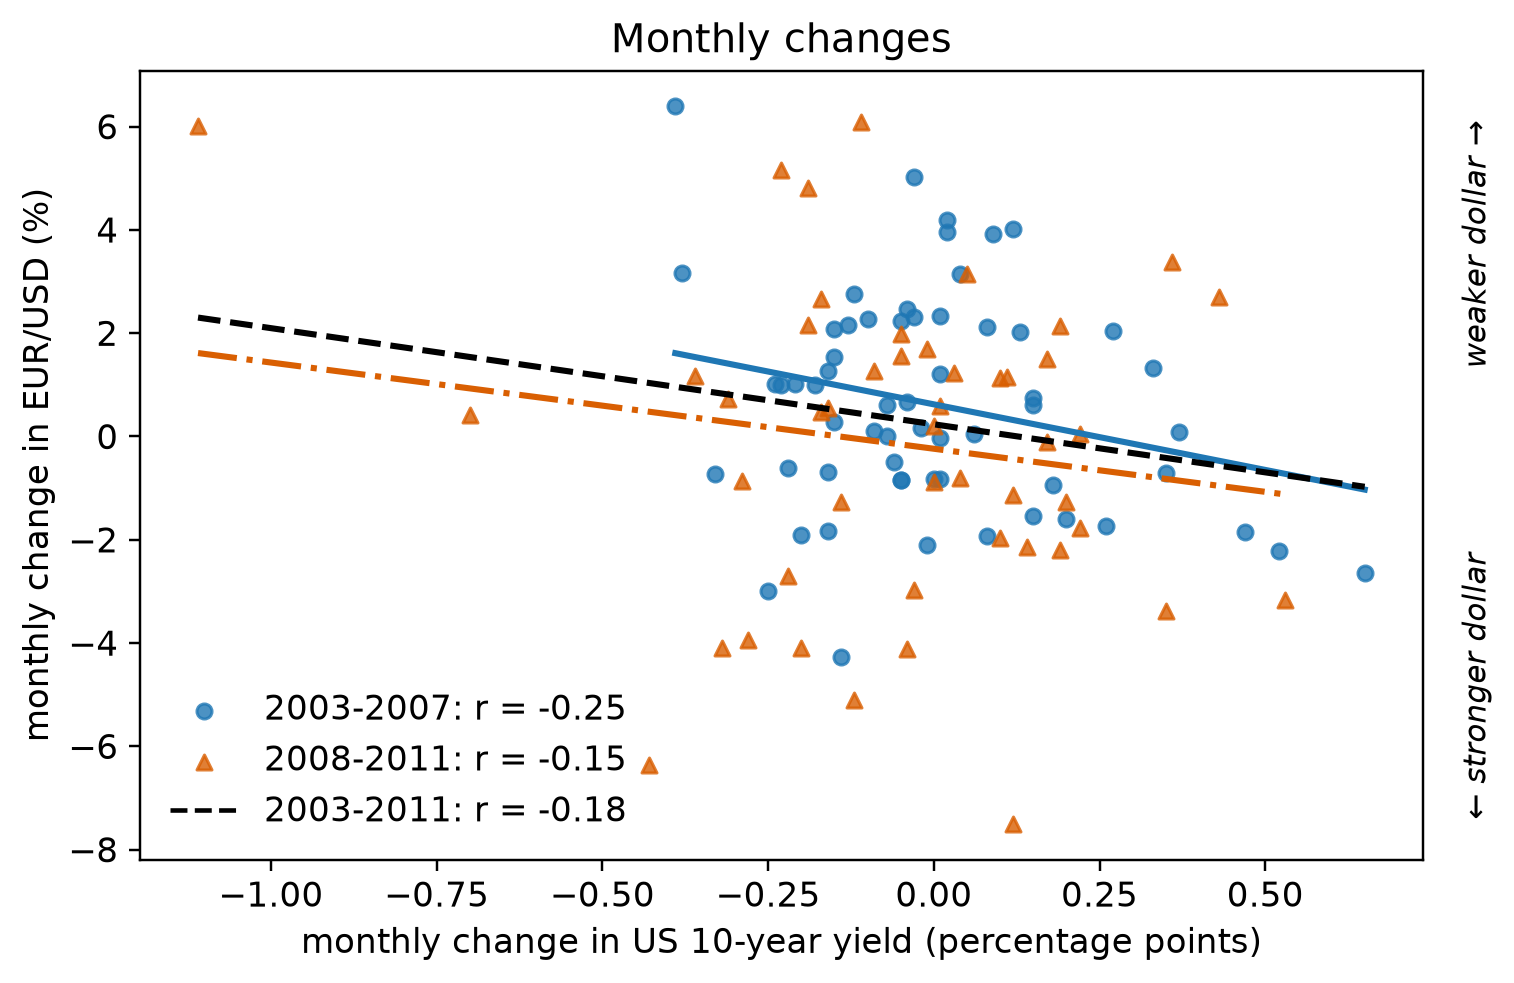
\includegraphics[width=0.74\textwidth]{../graphics/1-12CW_D_eurusd_us10y_3_changes_scatter.png}
\end{center}

\begin{enumerate}[itemsep=0.1cm]
  \item[(b)] Write down the three values of $r$ for the monthly changes.
  Compare them with your answers to 2(a).
  \vfill
  \item[(c)] In a month when the US yield rises, the investor's bonds lose
  value. Use the sign of $r$ to state what tends to happen to EUR/USD in
  that month, and explain how this affects the investor's total risk.
  \vfill
\end{enumerate}

\newpage

%--- Problem 4: Six-point Simpson's paradox on the GDC; why changes resist the paradox; why correlating price levels misleads in a research paper ---
%--- Source: Original (AA SL 4.4); whiteboard example from correlation_lesson_notes.md ---
\item[4.] A small data set shows the same effect.

\begin{center}
\setlength{\tabcolsep}{7pt}\renewcommand{\arraystretch}{1.15}
\begin{tabular}{|l|c|c|c|c|c|c|}
\hline
Period & \multicolumn{3}{c|}{1} & \multicolumn{3}{c|}{2} \\
\hline
$x$ & 1 & 2 & 3 & 6 & 7 & 8 \\
\hline
$y$ & 5 & 4 & 3 & 10 & 9 & 8 \\
\hline
\end{tabular}
\end{center}

\begin{enumerate}[itemsep=0.1cm]
  \item Find $r$ for period 1, for period 2, and for all six points.
  \vfill
  \item Sketch the six points. Explain the result of part (a).
  \vfill
  \item Prices tend to drift up or down over the years, so their average
  level is different in each period. Monthly changes average close to
  zero in every period. Explain why the correlation of changes is much
  less affected by Simpson's paradox than the correlation of levels.
  \vfill
  \item A research paper finds $r = 0.3$ between the prices of gold and oil
  from 2015 to 2025, but $r < 0$ in each half of the period. Write two
  sentences of advice to the author.
  \vfill
\end{enumerate}

\end{enumerate}
\end{document}
